% 第3章第4节：积分方程的可解性与稳定性（两类方程、小范数迭代、紧算子的Fredholm二择、第一类方程与小奇异值）。

\section{积分方程的可解性与稳定性}
\label{sec:ose-integral-equations}

前三节都在正向使用算子：给定输入，计算输出。本节反过来，把积分算子放进未知函数满足的方程，依次回答章首的三个问题：解是否存在、是否唯一、对数据的误差是否稳定。两类方程的像空间结构截然不同，所以分开处理：第二类方程在小范数条件下可以直接迭代求解，在紧性条件下有完整的可解性判别；第一类方程还要面对小奇异值带来的放大。

\subsection{第一类与第二类积分方程}
\label{sec:ose-equation-types}

\paragraph{两类方程}
设$T$是积分算子，$g$是已知函数，$f$是未知函数。若$T:H_1\to H_2$，方程
\begin{equation}
  Tf=g
  \label{eq:ose-first-kind}
\end{equation}
称为\term{第一类积分方程}（integral equation of the first kind），此时$g$是观察到的输出，要求恢复产生它的输入。若$T:H\to H$，$\lambda\in\mathbb F$为参数，方程
\begin{equation}
  (I-\lambda T)f=g,\qquad\text{即}\quad f(x)-\lambda\int K(x,z)f(z)\,d\mu(z)=g(x),
  \label{eq:ose-second-kind}
\end{equation}
称为\term{第二类积分方程}（integral equation of the second kind），此时$g$是源项，未知函数同时出现在积分内外。两类方程的区别不在于写法：第二类方程中，未知函数在积分之外还有一个单位算子的“副本”，这个副本保证了在积分算子看不见的方向上，信息不会丢失。

\paragraph{贯穿例子中的两类方程}
回到$L^2([-1,1],\mu)$、$d\mu=dz/2$、$K(x,z)=1+xz$。由第~\ref{sec:ose-spectral-theorem}小节，任意$f$可以分解为$f=\alpha+\beta x+h$，其中$h$与$1,x$都正交，并且$Tf=\alpha+\frac{\beta}{3}x$。

第一类方程$Tf=g$只能产生一次函数，所以只有当$g=a+bx$时才有解。此时$\alpha=a$、$\beta=3b$，而$h$完全不受约束：
\[
  f=a+3bx+h,\qquad h\perp1,\ h\perp x .
\]
解存在时有无穷多个，差别正是$\ker T$中的任意元素，这个核是无限维的。

第二类方程$(I-\lambda T)f=g$则不同。把$g$同样分解为$g=a+bx+k$，$k$与$1,x$正交，逐方向比较系数得
\[
  (1-\lambda)\alpha=a,\qquad\Bigl(1-\frac{\lambda}{3}\Bigr)\beta=b,\qquad h=k .
\]
只要$\lambda\neq1,3$，每个$g$都给出唯一解；例如$\lambda=1/2$时$f=2a+\frac65bx+k$。图~\ref{fig:ose-equation-types}比较两类方程在各方向上的乘子：第一类方程把与$1,x$正交的方向全部乘以零，第二类方程在这些方向上保留单位作用，只在两个特征方向上改变比例。

\begin{figure}[!htb]
  \centering
  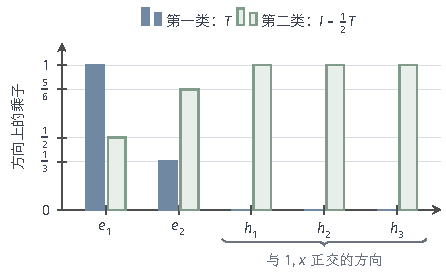
\includegraphics[width=75.5mm]{figures/02-abstract-mathematics/03-function-spaces/tikz/c3-equation-types/figure.pdf}
  \caption{核$1+xz$（测度$dz/2$）给出的两类方程在各正交方向上的乘子。$e_1=1$、$e_2=\sqrt3x$为特征方向，$h_1,h_2,h_3$代表与它们正交的方向（如$x^2-1/3$）。深色：第一类方程的算子$T$，在正交方向上为零，信息丢失；浅色：第二类方程的算子$I-\frac12T$，在正交方向上恒为$1$。}
  \label{fig:ose-equation-types}
\end{figure}

\paragraph{核、像与例外参数}
同一个例子已经显示出两类方程各自的困难。第一类方程的困难来自$T$本身：$\ker T$非零造成不唯一，$\operatorname{Ran}T$不是全空间造成不存在。第二类方程只在特殊参数处出问题：$\lambda=1$时齐次方程$(I-T)f=0$有非零解$f=1$，$\lambda=3$时有非零解$f=x$；这两个参数正是特征值$1$与$1/3$的倒数。

由此形成本节其余部分的分工。第~\ref{sec:ose-neumann}小节说明，当$\|\lambda T\|<1$时，第二类方程可以用级数和迭代直接构造解；第~\ref{sec:ose-fredholm}小节用紧性给出第二类方程对所有参数的可解性判别；第~\ref{sec:ose-first-kind}小节回到第一类方程，说明除了正交条件，还需要控制反演时被除掉的小奇异值。

\subsection{小范数条件下的解与迭代}
\label{sec:ose-neumann}

\paragraph{Neumann级数}
标量方程$(1-q)x=g$在$|q|<1$时有解$x=\sum_{n\geq0}q^ng$。算子方程可以照此办理，只要几何级数在算子范数下收敛。第~\ref{sec:lfo-operator-space}节已经证明，$X$为Banach空间时$\mathcal B(X)$在算子范数下完备，这正是让级数收敛所需要的。

\begin{theorem}[Neumann级数]
\label{thm:ose-neumann}
设$X$为Banach空间，$S\in\mathcal B(X)$且$\|S\|<1$。则$I-S$可逆，逆算子有界，并且
\[
  (I-S)^{-1}=\sum_{n=0}^{\infty}S^n,\qquad\|(I-S)^{-1}\|\leq\frac{1}{1-\|S\|},
\]
级数按算子范数收敛。
\end{theorem}

\begin{proof}
由$\|S^n\|\leq\|S\|^n$，级数$\sum_n\|S^n\|$被收敛的几何级数控制，部分和$P_N=\sum_{n=0}^{N}S^n$在$\mathcal B(X)$中是柯西列，由完备性收敛到某个$P$，且$\|P\|\leq\sum_n\|S\|^n=1/(1-\|S\|)$。部分和满足望远镜恒等式
\[
  P_N(I-S)=(I-S)P_N=I-S^{N+1},
\]
而$\|S^{N+1}\|\leq\|S\|^{N+1}\to0$。令$N\to\infty$，由算子乘法对算子范数连续，得$P(I-S)=(I-S)P=I$。
\end{proof}

由该级数定义的
\[
  \sum_{n=0}^{\infty}S^n
\]
称为\term{Neumann级数}（Neumann series）。取$S=\lambda T$，当$\|\lambda T\|<1$时，第二类方程~\eqref{eq:ose-second-kind}对每个$g$有唯一解$f=\sum_n\lambda^nT^ng$，且$\|f\|\leq\|g\|/(1-|\lambda|\|T\|)$。数据误差的影响由同一个界控制：若源项从$g$变为$\tilde g$，解的变化不超过$\|g-\tilde g\|/(1-\|\lambda T\|)$。

\paragraph{压缩迭代}
Neumann级数的部分和可以逐步计算。令$\Phi(f)=g+\lambda Tf$，则方程~\eqref{eq:ose-second-kind}等价于不动点方程$f=\Phi(f)$。从$f_0$出发迭代$f_{n+1}=\Phi(f_n)$，展开得
\[
  f_n=\sum_{k=0}^{n-1}(\lambda T)^kg+(\lambda T)^nf_0 ,
\]
即Neumann级数的部分和加上一项逐渐消失的初值影响。这个迭代满足本卷“度量空间”章压缩映射定理（定理~\ref{thm:metric-contraction}）的全部条件：$X$完备；$\Phi$把$X$映入自身；对任意$f,h$有
\[
  \|\Phi(f)-\Phi(h)\|=\|\lambda T(f-h)\|\leq q\|f-h\|,\qquad q=\|\lambda T\|<1 .
\]
压缩常数$q$对所有输入统一成立，这是压缩映射定理要求的，也是小范数条件提供的。

\paragraph{误差估计}
压缩映射定理的先验估计~\eqref{eq:metric-a-priori}直接给出
\[
  \|f_n-f_*\|\leq\frac{q^n}{1-q}\|f_1-f_0\| .
\]
若每步迭代都带有执行误差，即实际计算的$f_{n+1}$满足$\|f_{n+1}-\Phi(f_n)\|\leq\eta_n$，记$e_n=\|f_n-f_*\|$，第~\ref{sec:metric-inexact-contraction}节的递推~\eqref{eq:metric-inexact-error}给出$e_{n+1}\leq qe_n+\eta_n$。在$\eta_n\leq\eta$时，展开递推得到$\limsup_ne_n\leq\eta/(1-q)$：每步的执行误差被放大$1/(1-q)$倍，形成一个误差地板。$q$接近$1$时，即使每步误差很小，最终误差也可能很大。

\begin{example}[迭代求解第二类方程]
\label{ex:ose-neumann-iteration}
在贯穿例子中取$\lambda=1/2$，$g=1+x$。此时$q=\|\frac12T\|=\frac12$。由前一小节的系数关系，精确解为$f_*=2+\frac65x$。从$f_0=0$迭代，常数系数满足$a_{n+1}=1+\frac12a_n$，$x$的系数满足$b_{n+1}=1+\frac16b_n$，所以
\[
  a_n=2\bigl(1-2^{-n}\bigr),\qquad b_n=\tfrac65\bigl(1-6^{-n}\bigr),
\]
误差为
\[
  \|f_n-f_*\|^2=\bigl(2\cdot2^{-n}\bigr)^2+\tfrac13\bigl(\tfrac65\cdot6^{-n}\bigr)^2 .
\]
这里用到$\|\alpha+\beta x\|^2=|\alpha|^2+|\beta|^2/3$。先验界为$\frac{2^{-n}}{1/2}\|g\|=2\cdot2^{-n}\cdot\frac{2}{\sqrt3}$，比实际误差略大。若每步都多加一个$-10^{-3}$的常数偏差，常数系数改为收敛到$2-2\times10^{-3}$，误差停在$2\times10^{-3}=\eta/(1-q)$，恰好达到误差地板。
\end{example}

\begin{figure}[!htb]
  \centering
  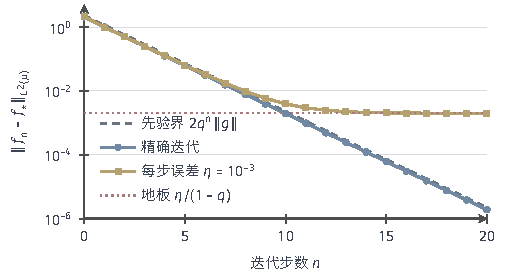
\includegraphics[width=85.7mm]{figures/02-abstract-mathematics/03-function-spaces/tikz/c3-neumann-error/figure.pdf}
  \caption{第二类方程$(I-\frac12T)f=1+x$（核$1+xz$，测度$dz/2$）的不动点迭代误差，纵轴取对数。虚线：先验界$q^n\|f_1-f_0\|/(1-q)$，$q=1/2$；圆点：精确迭代，误差几乎按$2^{-n}$下降；方点：每步带有大小$\eta=10^{-3}$的常数偏差，误差停在点线所示的地板$\eta/(1-q)=2\times10^{-3}$。}
  \label{fig:ose-neumann-error}
\end{figure}

图~\ref{fig:ose-neumann-error}画出例~\ref{ex:ose-neumann-iteration}的三条曲线。精确迭代的误差几乎贴着先验界下降，速度由最慢的方向$a_n$的比例$1/2$决定；带执行误差的迭代起初与精确迭代重合，大约十步后停在地板上，继续迭代不再改进。

\paragraph{小范数只是充分条件}
$\|\lambda T\|<1$保证可解，但不是可解的必要条件。最简单的例子是$B=2I$：$\|B\|=2$，Neumann级数$\sum_nB^n=\sum_n2^nI$发散，迭代$f_{n+1}=g+2f_n$从$f_0=0$出发给出$f_n=(2^n-1)g$，也发散；可是$I-B=-I$显然可逆，方程$(I-B)f=g$的唯一解为$f=-g$。这里的$B$不是用平方可积核表示的积分算子，只用来说明一般算子的情形。

积分方程中也有同样的现象。贯穿例子中取$\lambda=2$，则$\|\lambda T\|=2$，但$\lambda\neq1,3$，方程$(I-2T)f=g$对每个$g=a+bx+k$有唯一解$f=-a+3bx+k$。迭代的常数系数却满足$a_{n+1}=a+2a_n$，只要$a\neq0$就发散。方程可解与某个迭代法收敛是两件事；要判断前者，需要下一小节的工具。

\subsection{紧算子条件下的可解性}
\label{sec:ose-fredholm}

小范数条件把第二类方程限制在$|\lambda|<1/\|T\|$的范围内。对紧算子，我们能对所有参数给出完整的判别。先在紧自伴情形中用特征方向看清答案，再对一般紧算子给出证明。

\paragraph{紧自伴情形的方向解释}
设$T$为紧自伴算子，按定理~\ref{thm:ose-compact-selfadjoint}有特征对$(\lambda_j,e_j)$及$u=u_0+\sum_jc_je_j$，其中$u_0\in\ker T$，$c_j=\langle e_j,u\rangle$。则
\[
  (I-\lambda T)u=u_0+\sum_j(1-\lambda\lambda_j)c_je_j .
\]
$I-\lambda T$在核方向上作用为$1$，在第$j$个特征方向上乘以$1-\lambda\lambda_j$。若$\lambda$不等于任何$1/\lambda_j$，这些乘子都非零；又因为$\lambda_j\to0$，乘子趋于$1$，所以$\inf_j|1-\lambda\lambda_j|>0$。逐方向除以乘子就得到有界逆：
\[
  f=g_0+\sum_j\frac{\langle e_j,g\rangle}{1-\lambda\lambda_j}e_j ,\qquad g_0\text{为}g\text{在}\ker T\text{上的分量}.
\]
若$\lambda=1/\lambda_k$，乘子在$\lambda_k$的特征空间上为零，这个有限维特征空间就是齐次方程的解空间$\ker(I-\lambda T)$；方程可解当且仅当$g$在这些方向上的系数为零，即$g\perp\ker(I-\lambda T)$，此时解可以加上该特征空间中的任意元素。$\lambda$为实数，$I-\lambda T$自伴，所以这里的正交条件也就是$g\perp\ker(I-\lambda T)^*$。

图~\ref{fig:ose-fredholm-alternative}在贯穿例子上画出三个乘子随$\lambda$的变化。常数方向的乘子$1-\lambda$在$\lambda=1$处为零，线性方向的乘子$1-\lambda/3$在$\lambda=3$处为零，正交补方向的乘子恒为$1$。除这两个例外参数外，方程总是唯一可解的；$\lambda=1/2$与$\lambda=2$都在这个范围内，尽管只有前者满足小范数条件。

\begin{figure}[!htb]
  \centering
  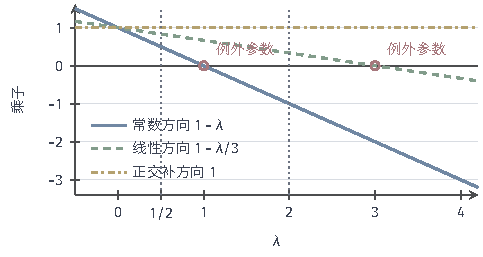
\includegraphics[width=81.8mm]{figures/02-abstract-mathematics/03-function-spaces/tikz/c3-fredholm-alternative/figure.pdf}
  \caption{第二类方程$(I-\lambda T)f=g$在各方向上的乘子随参数$\lambda$的变化（核$1+xz$，测度$dz/2$）。乘子为零的$\lambda=1$与$\lambda=3$（空心圆）是例外参数，齐次方程在此有非零解；其余参数下方程唯一可解。点线标出$\lambda=1/2$（满足小范数条件）与$\lambda=2$（不满足，但仍唯一可解）。}
  \label{fig:ose-fredholm-alternative}
\end{figure}

\paragraph{Fredholm二择定理}
对一般紧算子，没有正交特征基可用，但结论的形式保持不变。

\begin{theorem}[Fredholm二择定理]
\label{thm:ose-fredholm}
设$H$为Hilbert空间，$T:H\to H$为紧算子，$\lambda\in\mathbb F$，$B=I-\lambda T$。则：
\begin{enumerate}
  \item $\ker B$与$\ker B^*$都是有限维的；
  \item $\operatorname{Ran}B$是闭子空间，因而$\operatorname{Ran}B=(\ker B^*)^\perp$；
  \item $\ker B=\{0\}$当且仅当$\operatorname{Ran}B=H$，此时$B^{-1}$有界。
\end{enumerate}
因此以下二者恰有一个成立：齐次方程$Bf=0$只有零解，此时对每个$g\in H$，方程$Bf=g$有唯一解，且解有界地依赖于$g$；或者齐次方程有非零解，此时$Bf=g$可解当且仅当$g\perp\ker B^*$，全部解为一个特解加上$\ker B$中的任意元素。
\end{theorem}

这个结论称为\term{Fredholm二择定理}（Fredholm alternative）。它的力量在于第二条：像空间闭合是事先由紧性保证的，所以正交条件$g\perp\ker B^*$判断的是\emph{精确}可解，而不只是$g$能否被输出逼近。对比第~\ref{sec:lfo-range-kernel}节中的$A(x_n)=(x_n/n)$：$\ker A^*=\{0\}$，每个$y$都满足正交条件，但$(1/n)$并不在像中，因为$\operatorname{Ran}A$不闭。还可以证明$\dim\ker B=\dim\ker B^*$，这里不需要这一结论，不再展开。

\paragraph{证明思路：有限秩加小范数余项}
证明把紧算子拆成两部分：有限秩部分化为有限维线性方程组，余项部分用Neumann级数吸收。$\lambda=0$时$B=I$，结论显然，下面设$\lambda\neq0$。

\begin{proof}
第一步，分解。由定理~\ref{thm:ose-finite-rank-approx}，取有限秩算子$F$使$\|\lambda(T-F)\|<1$。记$C=I-\lambda(T-F)$，由定理~\ref{thm:ose-neumann}，$C$可逆且$C,C^{-1}$都有界。于是
\[
  B=C-\lambda F=C(I-G),\qquad G=\lambda C^{-1}F .
\]
$G$仍是有限秩算子。取$\operatorname{Ran}G$的一组线性无关基$b_1,\ldots,b_r$，则$Gf=\sum_{i=1}^r\ell_i(f)b_i$，系数$\ell_i$是有界线性泛函，由Riesz表示（第~\ref{sec:lfo-riesz}节）写成$\ell_i(f)=\langle a_i,f\rangle$。

第二步，化为矩阵方程。令$\bm M_{i,j}=\langle a_i,b_j\rangle$，$\bm d(h)=(\langle a_1,h\rangle,\ldots,\langle a_r,h\rangle)^\top$。我们断言：$(I-G)f=h$当且仅当$f=h+\sum_ic_ib_i$，其中$\bm c=(c_1,\ldots,c_r)^\top$满足$(\bm I-\bm M)\bm c=\bm d(h)$。若$(I-G)f=h$，则$f=h+Gf=h+\sum_ic_ib_i$，其中$c_i=\langle a_i,f\rangle=\langle a_i,h\rangle+\sum_j\bm M_{i,j}c_j$。反过来，若$\bm c$满足矩阵方程，令$f=h+\sum_jc_jb_j$，则$Gf=\sum_i\bigl(\bm d(h)_i+(\bm M\bm c)_i\bigr)b_i=\sum_ic_ib_i=f-h$。

第三步，核有限维、像闭合。取$h=0$，$\ker(I-G)$由$\ker(\bm I-\bm M)$经单射$\bm c\mapsto\sum_ic_ib_i$得到，维数不超过$r$；$C$可逆，所以$\ker B=\ker(I-G)$有限维。由第二步，$h\in\operatorname{Ran}(I-G)$当且仅当$\bm d(h)\in\operatorname{Ran}(\bm I-\bm M)$。$\mathbb F^r$的子空间$\operatorname{Ran}(\bm I-\bm M)$是有限个线性泛函的公共零点，与连续映射$\bm d$复合后，$\operatorname{Ran}(I-G)$是$H$上有限个连续线性泛函的公共零点，因而闭。$C$与$C^{-1}$都连续，所以$\operatorname{Ran}B=C\bigl(\operatorname{Ran}(I-G)\bigr)$也闭。

第四步，单射推出满射。若$\ker B=\{0\}$，则$\ker(\bm I-\bm M)=\{0\}$，有限维方阵$\bm I-\bm M$可逆，矩阵方程对每个$\bm d(h)$有解，于是$I-G$满射，$B=C(I-G)$也满射。反之，若$B$满射，则$\ker B^*=(\operatorname{Ran}B)^\perp=\{0\}$；对下一步说明的紧算子$T^*$应用本步，$B^*$满射，从而$\ker B=(\operatorname{Ran}B^*)^\perp=\{0\}$。双射$B$的逆有界由第~\ref{sec:lfo-open-mapping}节的有界逆定理保证。

第五步，处理伴随。若$F_n$是有限秩算子且$\|T-F_n\|\to0$，则$F_n^*$也是有限秩的（$F_nf=\sum_i\langle a_i,f\rangle b_i$时$F_n^*g=\sum_i\langle b_i,g\rangle a_i$），且$\|T^*-F_n^*\|=\|T-F_n\|\to0$，由定理~\ref{thm:ose-compact-limit}，$T^*$是紧算子。$B^*=I-\overline\lambda T^*$与$B$同型，由第三步，$\ker B^*$有限维。最后，像闭合且由第~\ref{sec:lfo-range-kernel}节$\overline{\operatorname{Ran}B}=(\ker B^*)^\perp$，得$\operatorname{Ran}B=(\ker B^*)^\perp$。
\end{proof}

第三步中，有限维的矩阵方程决定了无限维方程的全部可解性：无限维部分已经被可逆的$C$吸收。这也说明了紧性的作用：若$T$不能被有限秩算子逼近，就无法把问题化到有限维。

\paragraph{两个推论}
定理的第三条有一个直接推论：紧算子$T$的非零谱点都是特征值。若$\mu\neq0$不是特征值，取$\lambda=1/\mu$，则$I-\lambda T$是单射，由定理是有界可逆的，于是$T-\mu I=-\mu(I-\lambda T)$也有界可逆，$\mu\in\rho(T)$。结合第~\ref{sec:ose-spectrum-def}小节，无限维空间中紧算子的谱由至多可数个非零特征值和$0$组成。

另一个推论关于迭代。Fredholm二择告诉我们方程何时可解，但没有给出求解的迭代格式。第~\ref{sec:ose-neumann}小节中$\lambda=2$的例子正处于“唯一可解但迭代发散”的情形：定理~\ref{thm:ose-fredholm}保证解存在、有界依赖于数据，固定点迭代仍受$\|\lambda T\|<1$的收缩条件限制。

\subsection{第一类方程与小奇异值}
\label{sec:ose-first-kind}

第一类方程$Tf=g$没有单位算子的“副本”，紧算子$T$的像一般不闭，Fredholm二择的结论不再适用。本小节用奇异值分解给出精确可解的条件，并说明为什么即使解存在，它也可能对数据极其敏感。

\paragraph{精确可解的Picard条件}
设$T:H_1\to H_2$为紧算子，奇异值分解为$Tx=\sum_j\sigma_j\langle v_j,x\rangle u_j$。若$Tf=g$，则对每个$j$，
\[
  \langle u_j,g\rangle=\langle u_j,Tf\rangle=\langle T^*u_j,f\rangle=\sigma_j\langle v_j,f\rangle ,
\]
所以$f$在$v_j$方向上的系数只能是$\langle u_j,g\rangle/\sigma_j$。这些系数必须平方可和，$f$才属于$H_1$。

\begin{theorem}[第一类方程的可解性与最小范数解]
\label{thm:ose-picard}
设$T:H_1\to H_2$为紧算子，奇异值分解如定理~\ref{thm:ose-svd}。则$Tf=g$有解，当且仅当以下两条同时成立：
\begin{equation}
  g\perp\ker T^*,\qquad \sum_j\frac{|\langle u_j,g\rangle|^2}{\sigma_j^2}<\infty .
  \label{eq:ose-picard}
\end{equation}
此时
\[
  f^\dagger=\sum_j\frac{\langle u_j,g\rangle}{\sigma_j}v_j
\]
是唯一属于$(\ker T)^\perp$的解，全部解为$f^\dagger+\ker T$，且$f^\dagger$是范数最小的解。
\end{theorem}

\begin{proof}
必要性：若$Tf=g$，则$g\in\operatorname{Ran}T\subseteq(\ker T^*)^\perp$；由上面的系数关系和Bessel不等式，$\sum_j|\langle u_j,g\rangle|^2/\sigma_j^2=\sum_j|\langle v_j,f\rangle|^2\leq\|f\|^2$。

充分性：第二个条件使级数$f^\dagger$按范数收敛（第~\ref{sec:fs-orthogonal-expansion}节），且$f^\dagger$属于$(v_j)$的闭张成$(\ker T)^\perp$。由连续性逐项作用，$Tf^\dagger=\sum_j\langle u_j,g\rangle u_j$，这是$g$在$(u_j)$的闭张成上的正交投影。由定理~\ref{thm:ose-svd}，这个闭张成等于$(\ker T^*)^\perp$，而第一个条件说明$g$就在其中，所以$Tf^\dagger=g$。

解的结构：两个解之差属于$\ker T$，故全部解为$f^\dagger+\ker T$。$(\ker T)^\perp$中的解唯一，因为两个这样的解之差同时属于$\ker T$与$(\ker T)^\perp$。对任意解$f=f^\dagger+h$，$h\in\ker T$与$f^\dagger$正交，由勾股定理$\|f\|^2=\|f^\dagger\|^2+\|h\|^2\geq\|f^\dagger\|^2$。
\end{proof}

式~\eqref{eq:ose-picard}中的第二个条件称为\term{Picard条件}（Picard condition），$f^\dagger$称为\term{最小范数解}（minimum-norm solution）。两个条件分工不同：第一个只保证$g$位于像的闭包中，即$g$能被输出任意逼近；第二个才保证形式逆像$\sum_j\sigma_j^{-1}\langle u_j,g\rangle v_j$真正属于输入空间。

\paragraph{Picard条件的例子}
在贯穿例子中，$T$只有两个奇异值$1$与$1/3$，Picard条件自动成立，第一个条件就是$g\in\operatorname{span}\{1,x\}$；对$g=a+bx$，最小范数解为$f^\dagger=a+3bx$，与第~\ref{sec:ose-equation-types}小节的结果一致，它正是全部解中去掉核分量$h$的那一个。

$\ell^2$上的$A(x_n)=(x_n/n)$说明两个条件确实不同。$A$自伴且单射，$\ker A^*=\{0\}$，第一个条件对所有$g$成立；奇异值$\sigma_n=1/n$，Picard条件化为$\sum_nn^2|g_n|^2<\infty$。图~\ref{fig:ose-picard-coefficients}比较两组数据：$g^{(1)}_n=1/n^2$的形式解系数为$1/n$，平方可和，$g^{(1)}=A(1/n)$；$g^{(2)}_n=1/n$本身平方可和，但形式解系数恒为$1$，不平方可和，所以$g^{(2)}$不在像中。这正是第~\ref{sec:lfo-range-kernel}节的例子，现在由Picard条件统一解释。

\begin{figure}[!htb]
  \centering
  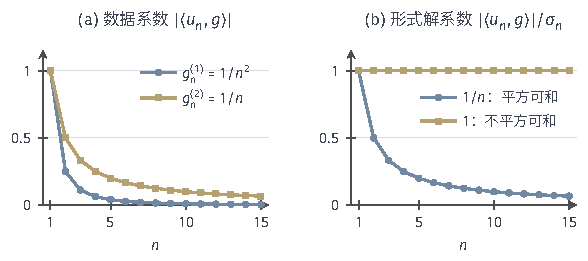
\includegraphics[width=99.6mm]{figures/02-abstract-mathematics/03-function-spaces/tikz/c3-picard-coefficients/figure.pdf}
  \caption{$\ell^2$上$A(x_n)=(x_n/n)$的Picard条件。(a) 两组数据的系数$1/n^2$与$1/n$，都平方可和，都满足$g\perp\ker A^*$。(b) 除以奇异值$\sigma_n=1/n$后的形式解系数：前者为$1/n$，平方可和，方程可解；后者恒为$1$，不平方可和，方程无解。}
  \label{fig:ose-picard-coefficients}
\end{figure}

对例~\ref{ex:ose-volterra-svd}的积分算子$V$，若$g$绝对连续、$g(0)=0$且$g'\in L^2(0,1)$，分部积分并利用$\cos\omega_k=0$可得$\langle u_k,g\rangle=\sigma_k\langle v_k,g'\rangle$，于是Picard级数等于$\sum_k|\langle v_k,g'\rangle|^2=\|g'\|^2$，最小范数解就是$f^\dagger=g'$。求解第一类方程$Vf=g$就是求导，这与微分运算的不稳定性一致。

\paragraph{小奇异值放大扰动}
即使解存在，它对数据的依赖也可能没有统一的界。设$T$有无限多个正奇异值，$\sigma_j\to0$。取数据扰动$\delta g_j=\sigma_ju_j$，则$\|\delta g_j\|=\sigma_j\to0$；它满足Picard条件，相应的最小范数解扰动为
\[
  \delta f_j=\frac{\langle u_j,\delta g_j\rangle}{\sigma_j}v_j=v_j,\qquad\|\delta f_j\|=1 .
\]
数据误差趋于零，解的误差却始终为$1$。所以映射$g\mapsto f^\dagger$在$\operatorname{Ran}T$上无界；这也说明$\operatorname{Ran}T$不闭，否则$T$限制在$(\ker T)^\perp$上是到闭像的有界双射，由有界逆定理其逆有界。只有有限多个正奇异值时情况相反：$\|f^\dagger\|\leq\|g\|/\sigma_{\min}$，在贯穿例子中放大倍数至多为$3$。

\begin{figure}[!htb]
  \centering
  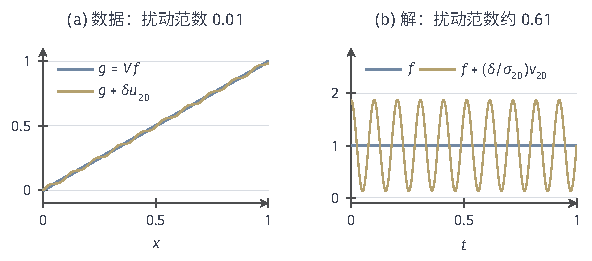
\includegraphics[width=100.2mm]{figures/02-abstract-mathematics/03-function-spaces/tikz/c3-noise-amplification/figure.pdf}
  \caption{第一类方程$Vf=g$（$(Vf)(x)=\int_0^xf$）中小奇异值放大扰动。真解$f=1$，数据$g=x$。(a) 数据加上范数为$0.01$的扰动$\delta u_{20}$，与原数据几乎重合。(b) 相应的最小范数解多出$(\delta/\sigma_{20})v_{20}$，振幅约$0.87$、范数约$0.61$，放大倍数$1/\sigma_{20}=19.5\pi\approx61$。}
  \label{fig:ose-noise-amplification}
\end{figure}

图~\ref{fig:ose-noise-amplification}在积分算子$V$上展示这一机制。数据中加入$\delta u_{20}$，$\delta=0.01$，曲线上几乎看不出差别；解中却多出振幅接近$0.87$的快速振荡。原因正是图~\ref{fig:ose-svd-decay}中看到的：$V$把快速振荡的输入平均掉，反解时必须把同样的振荡放大回去，振荡越快，放大倍数$1/\sigma_k=(k-\frac12)\pi$越大。

因此，第一类方程的解是否稳定，取决于数据在小奇异值方向上的成分。实际数据总带有误差，误差在所有方向上都有成分，直接计算$f^\dagger$会把高阶方向上的误差放大到失去意义。处理办法是舍去或压低小奇异值方向，例如只保留前$m$个奇异方向，或在求解目标中加入惩罚项；这些方法如何选择截断位置或惩罚强度、怎样平衡偏差与误差放大，属于优化问题，可参考\BookChapterRef{chap:optimization}{卷三“优化问题的定义与基本性质”章}及其后各章。从带噪观测中重建信号的具体任务，可参考\BookChapterRef{chap:signal-analysis}{卷三“信号”章}。
